\begin{center}
\scriptsize
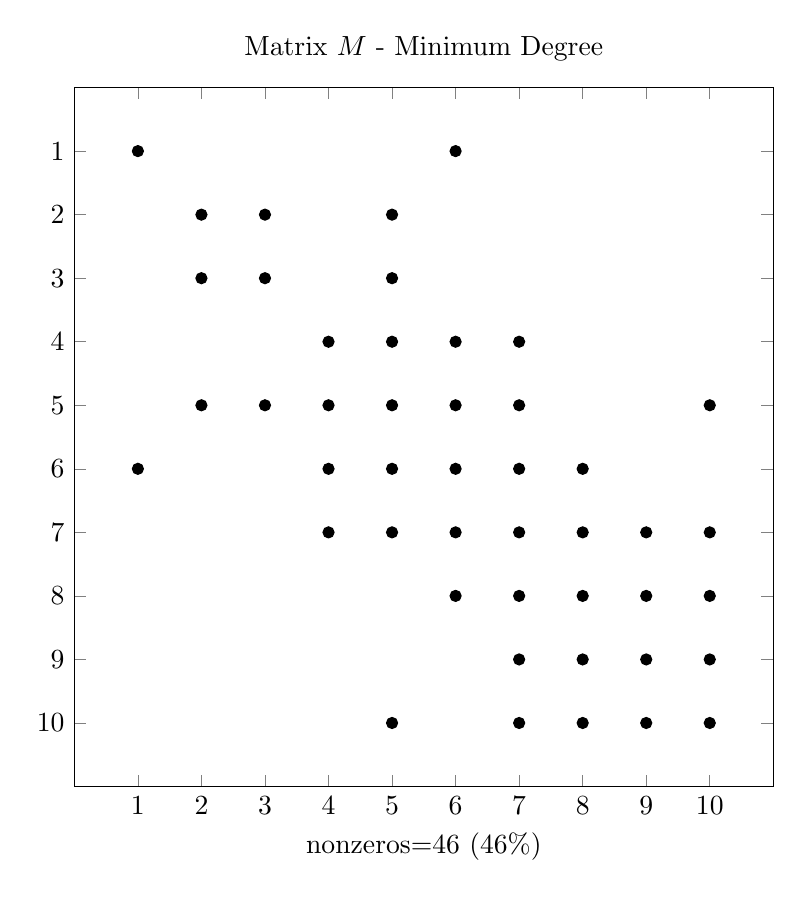
\begin{tikzpicture}
    [   baseline = {(current bounding box.north)}
    ]
    \begin{axis}
        [   unit vector ratio* = 1 1 1
        ,   y dir = reverse
        ,   xmin = 0
        ,   ymin = 0
        ,   xmax = 11
        ,   ymax = 11
        ,   title = {Matrix $M$ - Minimum Degree}
        ,   xlabel = {nonzeros=46 (46\%)}
        ,   width = \linewidth
        ,   xtick = {1,2,3,4,5,6,7,8,9,10}
        ,   ytick = {1,2,3,4,5,6,7,8,9,10}
        ]
        \addplot[only marks] coordinates
        {   (1,1)                    (6,1)
                 (2,2)(3,2)     (5,2)
                 (2,3)(3,3)     (5,3)
                           (4,4)(5,4)(6,4)(7,4)
                 (2,5)(3,5)(4,5)(5,5)(6,5)(7,5)          (10,5)
            (1,6)          (4,6)(5,6)(6,6)(7,6)(8,6)
                           (4,7)(5,7)(6,7)(7,7)(8,7)(9,7)(10,7)
                                     (6,8)(7,8)(8,8)(9,8)(10,8)
                                          (7,9)(8,9)(9,9)(10,9)
                                (5,10)  (7,10)(8,10)(9,10)(10,10)
        };
    \end{axis}
\end{tikzpicture}
\end{center}
